\chapter{Background}

Before presenting the design and implementation of a new approach to CPU modes this chapter
will give some background information about CPU modes, their definition and how
they are used currently. This section will also give a brief explanation
of the RISC-V architecture and the gem5 simulator, which are later used to implement
and simulate some of the designs. 

\section{CPU Modes}
In the dynamic world of computing, the central processing unit (CPU) is the core
of any digital system. An essential aspect of modern CPUs is the distinction
between operating modes. These modes play a critical role in efficient resource
management, enabling multitasking, and enhancing security in today's computing
systems.\par
While the most well-known examples of these modes are user and kernel mode,
recent years have witnessed the emergence of additional modes tailored to
specific scenarios. These include Hypervisor modes to facilitate
hardware-supported virtualization, monitor modes to establish isolated security
contexts, and more. Manufacturers like Intel (with technologies such as SGX and
MPK) and ARM (with TrustZone) have already incorporated these modes into their
CPUs. Given this evolving landscape, there is a need for a broader understanding
of modes and mode switches.\par
To grasp the concept of modes, it's essential to first comprehend how a CPU
executes software at an abstract level. Imagine a CPU as a canvas, and all
software that runs on it is represented by an instruction stream. This stream is
consumed and interpreted by the CPU, effectively programming it. Throughout this
process, internal components like Arithmetic Logic Units (ALUs) and load-store
units are invoked, leading to changes in the CPU's state. These changes can be
seen as the execution of a program. Roitzsch et al.\cite{Roitzsch} refer to this part of the
CPU as the ``data plane" since it influences the program's state in memory.
A set of execution semantics, definied by the behaviour of the components in the
data plane, can be seen as a mode.\par
The paper introduce another component called the ``control plane", which represents
the logic governing how the CPU modifies the program's state in memory. Unlike the
modular building blocks in the data plane, the control plane tends to be
complex, and hardwired. A mode switch, represented by the control plane,
signifies a stateful transition to the semantics of the data plane. These
semantics can vary in their impact on the system, with access to more robust
semantics often considered a privilege. Consequently, modes are sometimes
referred to as privilege levels, and mode switches are termed privilege
elevation. In the following sections, I will illustrate this definition with
examples, exploring Memory Protection Keys, x86 protection rings, and ARM's TrustZone,
applying this concept at various levels of abstraction, from minor memory
protections to comprehensive system-level transformations.\par

\subsection{Memory Protection Keys}
Memory Protection Keys (MPK) represent a notable feature available in x86
processors. When activated, MPK leverages four previously unused bits within
each page-table entry to encode one of sixteen keys. Each page can be tagged
with one of these keys. By setting the "write disable" bit for a particular key,
all attempts to write to a page with that key value are blocked, and setting the
"access disable" bit also prevents reads \cite{Corbet}. These keys can be assigned to
different threads, and if a thread attempts to access a page with a mismatched
key, it triggers a segmentation fault. To modify permissions for various pages,
only the permissions associated with the corresponding key need to be changed.
Such changes can be done by everyone which means that MPK can only be used to
protect against mistakes and not againgst attacks. This approach saves us from
the overhead of altering individual page-table entries and invalidating the
Translation Lookaside Buffers (TLBs).\par
This feature exemplifies the utility of defining modes and mode switches as sets
of semantics and stateful changes to those semantics. Under this definition,
this feature neatly fits. A thread and a page-table equipped with a protection
key collectively determine the semantics, particularly regarding memory access.
The assignment or alteration of such a key represents a shift in these
semantics, effectively changing how memory access is governed. 

\subsection{Protection Rings for x86 Processors}
The x86 architecture offers a protective mechanism that operates in conjunction
with both segmentation and paging techniques\cite{Intel}. This mechanism defines four
privilege levels, numbered from 0 to 3, with lower numbers indicating higher
privilege. Figure \ref{fig:x86} illustrates how these levels are organized as rings.
Only levels 0 and 3 are utilized due to the structure of most modern operating
systems. Specific CPU registers can only be written to at certain privilege
levels through special instructions. Attempting to use these instructions at an
insufficient privilege level would result in an exception.\par
Paging-level protection can be activated alongside the  segmentation approach or used in a
flat memory model where segment boundaries are set to the maximum and minimum
addresses. In this scenario, code and data segments must be configured for at
least rings 0 and 3. During page-level protection, rings 0, 1, and 2 are
considered kernel mode, while ring 3 is designated as user mode. In kernel mode,
all pages are accessible, while in user mode, access is limited to user mode
pages.\par
\begin{figure}[h]
    \centering
    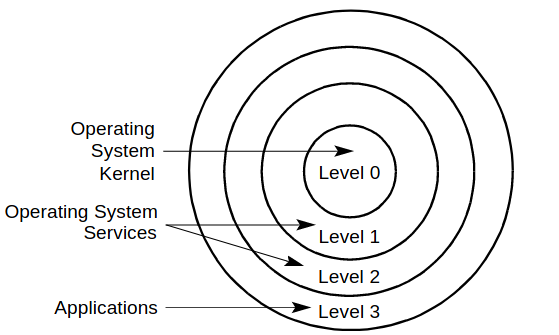
\includegraphics[width=0.5\textwidth]{protection_ring}
    \caption{Protection rings in x86}
    \label{fig:x86}
\end{figure}
In the segmentation approach, memory is divided into multiple segments, with the
most critical ones being the code segment, data segment, and stack segment. Each
segment has its own selector, which is employed to calculate the correct address
by selecting the appropriate segment descriptor from the Global or Local
Descriptor Table (GDT/LDT).The selector can be set by the application while the
descriptor can only be changed by the operating system and is hidden for the
application. These descriptors include a two-bit field known as
Descriptor Privilege Level (DPL), indicating the privilege level that can access
the segment. The CPU stores the Current Privilege Level (CPL) in a register for
segment selectors. Before any other checks, CPL and DPL are compared. If CPL is
equal to or smaller than DPL, access to the memory location is granted, allowing
higher privilege levels to access lower privilege level memory. Otherwise, the
processor generates a general-protection exception. In the event of an
exception, a handler routine is invoked, identified by a segment selector
pointing to a segment descriptor in the GDT or LDT for an executable code
segment. This handler routine may execute at the same privilege level as the
current code segment, as indicated by the DPL of the code segment. If the
privilege levels differ, the stack selector is altered, and CPL is updated to
the new privilege level. This enables the handler to operate at the higher
privilege level.\par
In this context, we can also observe how the concept of modes aligns with
execution semantics. The protection rings embody this semantics by reacting
differently to memory access. In one ring, access is granted, resulting in a
specific state change that we perceive as program execution. In another ring,
the same access or instruction might trigger an exception, leading to a
different state change. The mode switch, as a stateful change of
these semantics, is evident in the update of CPL, which influences the outcome
of the DPL vs. CPL check and consequently the execution of the code. This
underscores the need to reconfigure certain hardware components to establish a
fully software-based mode system. 

\subsection{ARM TrustZone}
TrustZone is a hardware security extension designed for ARM processors \cite{Pinto}. It
serves as an implementation of the Trusted Execution Environment concept. The
primary objective of TrustZone is to partition a processor into two distinct
states: the non-secure mode, which imposes certain restrictions, and the secure
mode, where restrictions are lifted as depicted in Figure \ref{fig:ARM}. This division
operates independently of other ARM modes, meaning that both states support the
usual modes for running an operating system. There are two exceptions to this
rule: the monitor mode, available exclusively in the secure state, and the
hypervisor mode, exclusive to the non-secure state. The monitor mode facilitates
transitions between these two states. In the non-secure state, this mode can
only be accessed through interrupts or the \texttt{SMC} instruction. It is possible to
determine whether an interrupt should trigger a switch to the secure state or be
handled in the IRQ mode within the non-secure state.\par
To implement TrustZone, the entire System-On-Chip (SoC) is divided into these
two distinct states. Isolation can be achieved physically or virtually. For
example, the processor can be time-shared between the two states, giving both
states the illusion of exclusive ownership \cite{ARM}. All hardware components,
including the Level 3 Cache, Memory Controller, DMA controller, and an AXI to
APB Bridge, are interconnected via an AXI bus. This bus incorporates an
active-high non-secure bit (NS). The NS bit is set whenever a memory request has
the Non-Secure Table Identifier (NSTID) bit set, which is the 33rd bit added to
every memory request. It signifies whether the processor is operating in the
secure or non-secure state. Most devices connected to the AXI bus behave
differently based on the NS bit. For instance, the MMU has two virtual MMUs (one
for each mode). The non-secure MMU can only map non-secure memory pages, while
the secure MMU can map all pages. The MMU utilizes a single TLB that employs
tags to differentiate between translations in the two states \cite{ARM}. Caches function
in a similar manner. It's important to note that this is a high-level
description of how these components work, as their operation is highly dependent
on the specific hardware implementation.\par
\begin{figure}[h]
    \centering
    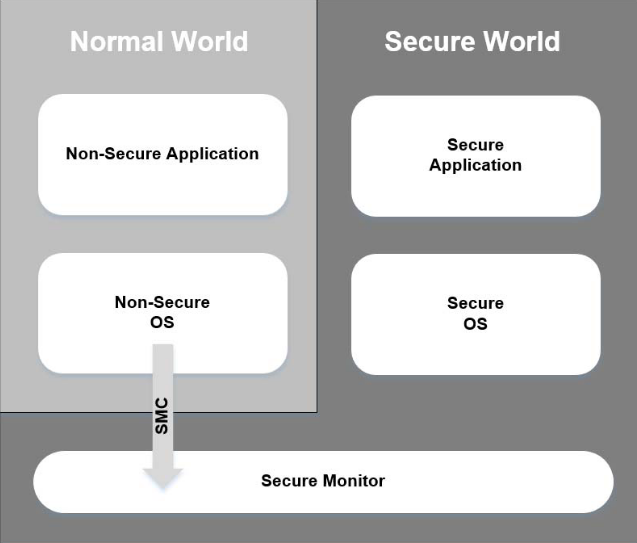
\includegraphics[width=0.7\textwidth]{armtrustzone}
    \caption{TrustZone}
    A division into normal world and secure world is done via hardware on a
    shared processor. Here shown for the ARM Cortex-A architecture.
    \label{fig:ARM}
\end{figure}
This example also illustrates the concept of modes and mode switches. The state
represents a mode and, consequently, an execution semantics. The transition from
one state to another represents a change in these semantics, which can be
interpreted as a mode switch. In this case, the alteration in semantics is more
apparent because it involves a tangible hardware change. In this scenario, the
AXI bus is reconfigured, leading to different interactions with connected
devices or triggering different functions within a device. Trusted Execution
Environments demonstrate the value of adopting a broader definition for modes
and mode switches. With the redesign of software-defined CPU modes, the aim is
to make it feasible to define such environments through software configurations.\par

\section{The RISC-V Architecture}
RISC-V, an open-source Instruction Set Architecture (ISA), has garnered
considerable attention due to its simplicity, versatility, and scalability\cite{Waterman_2}.
Developed at the University of California, Berkeley, RISC-V offers a modular and
extensible framework that caters to a diverse range of computing applications,
from embedded systems to high-performance servers. The choice of RISC-V as the
development platform in this work is motivated by its open-source nature and
relative architectural simplicity compared to x86 or ARM.

\subsection{Privilege Levels}
In traditional processor architectures, CPU modes are typically predefined as
fixed modes, such as kernel mode, user mode, and system mode. However, RISC-V
introduces a more adaptable approach through the concept of privilege levels.
Ranging from M-mode (Machine mode) at the highest privilege to U-mode (User
mode) at the lowest, RISC-V allows for the inclusion of optional S-mode
(Supervisor mode) and H-mode (Hypervisor mode) to address specific use cases.
This flexibility aligns well with the requirements of this work, which deals
with customizability at the hardware level.\par
Privilege levels in RISC-V are realized as distinct hardware extensions, each
bringing its own set of registers and instructions, as described by Waterman et
al.\cite{Waterman}. Moreover, RISC-V can employ various extensions to implement virtual
memory, ensuring memory-level separation. These extensions differ primarily in
the number of page table layers, with this work focusing on the 39-bit virtual
addresses.

\subsection{Privilege Elevation Mechanism}
RISC-V architecture relies on an exception handling mechanism to manage
privilege elevation. Exceptions, deviations from the normal program flow caused
by events like system calls, page faults, or hardware interrupts, trigger
privilege-level switches. \par
To facilitate privilege elevation, RISC-V introduces the "Trap-and-Return"
mechanism. Traps are synchronous exceptions triggered by specific instructions,
such as system calls or illegal instructions. When a trap occurs, the processor
switches to a higher privilege level and invokes a designated trap handler
routine to address the exception. Once the handler completes its task, it
employs the \texttt{mret} (Machine-level return) or \texttt{sret} (Supervisor-level return)
instruction to revert to the original privilege level. For asynchrounous
execeptions such as hardware interrupts the mechanism is the same.\par
Upon exception detection, the processor saves the current program counter (PC)
to the \texttt{mepc} register for machine-mode changes or the \texttt{sepc} register for
supervisor-mode changes. The type of exception is recorded in the \texttt{mcause} or
\texttt{scause} register, and interrupts are disabled by setting the \texttt{sie} bit in the
\texttt{mstatus} or \texttt{sstatus} register. The address of the corresponding trap handler routine is
stored in the \texttt{mtvec} or \texttt{stvec} register, depending on the processor's mode
change. The processor then switches to the target privilege level by
appropriately setting the relevant privilege-level bits in the \texttt{mstatus}
register.\par
During execution of the trap handler routine at the elevated privilege level,
the exception is handled accordingly. Necessary operations, such as servicing
the system call or resolving the page fault, are performed. Upon returning to
the lower privilege level, the processor restores the PC, allowing the program
to continue execution from where the exception occurred. However, tasks such as
saving register state and re-enabling interrupts are the responsibility of the
programmer.\par

\subsection{Memory Protection}
In the context of mode separation, memory protection plays a pivotal
role in ensuring isolation between different privilege levels. RISC-V
employs two distinct memory protection mechanisms: Physical Memory Protection
(PMP) and Paging. \par
PMP serves as a low-level protection mechanism, specifically designed to
safeguard certain regions of physical memory. It grants the Machine mode
exclusive control over configuring PMP settings. However, for the purpose of
this research, PMP's role is relatively minor, and thus, I focus my attention
on the more crucial memory protection mechanism: Paging.\par
Paging serves as the primary defense mechanism for safeguarding kernel memory
against unauthorized access from applications. The Sv39 RISC-V extension enables
this feature. While there are other extensions that support wider
virtual addresses, for the purpose of this thesis, I will concentrate on the
Sv39 extension due to its implementation in gem5 and only minor differences to
other extensions.\par
\begin{figure}[h]
    \centering
    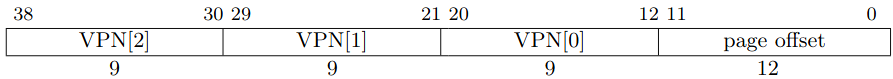
\includegraphics[width=\textwidth]{virtual_ad}
    \caption{Virtual Address}
    A 39-bit virtual address where every VPN[X] entry is an index for the
    corresponing PTE in the page table directory.
    \label{fig:virtad}
\end{figure}
The activation of the paging mechanism involves writing the address of the root
page table into the \texttt{satp} register. In the Sv39 extension, the page table
comprises three hierarchical levels which it's own page directory each. The virtual address undergoes division into
distinct parts (as shown in Figure \ref{fig:virtad}), indicating the index for a
page table entry (PTE) in a page directory. Figure \ref{fig:pte} illustrates a page
table entry with its status bits. The physical address (as shown in Figure
\ref{fig:pad}) is build from the PPN[X] parts of the PTE and the offset from the
virtual address. Any level can contain a leaf. This means Sv39 supports mega and
gigapages. If a such a pages occurs the missing PPN[X] parts in the PTE are
taken from the virtual address like PPN[X] = VPN[X]. Any errors during this
translation process raise a page-fault exception.\par
\begin{figure}[h]
    \centering
    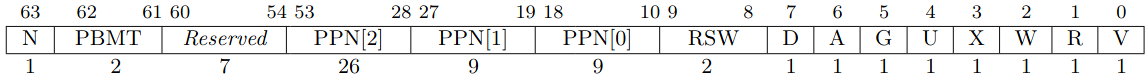
\includegraphics[width=\textwidth]{pte}
    \caption{Page Table Entry}
    A page table entry with various access rights bit at the end. The XWR bit
    indicating read, write and execution rights. If all this bits are zero the
    PTE is pointer to the next level. The V bit indicates if the page
    is valid while U shows if the page is accesible in user mode and G if it is
    a global mapping. Each PTE contains a access (A) and dirty (D) bit.
    \label{fig:pte}
\end{figure}
Each page table contains multiple permission bits, determining access rights to
a memory page. During translation they are checked. If a check fails a
page-fault exception is raised. These permission bits play a crucial role in controlling memory
access and will be expounded upon in detail in the design and implementation
chapter, as they undergo extensive changes throughout the research.\par
\begin{figure}[h]
    \centering
    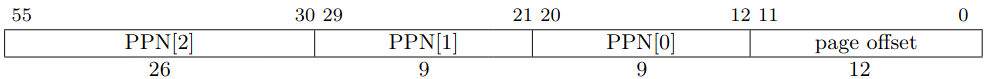
\includegraphics[width=\textwidth]{physical_ad}
    \caption{Physical Address}
    A physical address where the page offset is equal to the offset in the
    virtual address. The PPN[X] either given by the VPN[X] parts of the virtual
    address if it is a mega or gigapage or by the PTE.
    \label{fig:pad}
\end{figure}

\section{The gem5 Simulator}
The gem5 simulator\cite{gem5} stands as a modular full-system simulator,
renowned for its support of diverse instruction-set architectures and hardware
components. Employing a Python interface to interact with hardware components
written in C++, gem5 facilitates the construction of entire systems. This is
achieved by establishing connections between components through ports, enabling
seamless communication via packets exchanged among these interconnected
elements.
The inherent flexibility of gem5 allows for facile modification of packet
handling through alterations in the C++ implementation of objects. This, coupled
with its modular design, expedites the development process, facilitating swift
changes to the Instruction Set Architecture (ISA).
Crucially, for this thesis, gem5 operates on an event-driven model, empowering
precise timing in simulations. Events within gem5 correspond to granular stages,
such as instruction fetch, decode, and execute cycles, facilitating an accurate
simulation down to the timing of individual instructions. This capability to
model specific instructions and actions with precise timings enables a
accurate analysis of design overheads proposed in this thesis

\chapter{Related Work}

This thesis is the continuation of prior work and thoughts on the same and
similar topics. It was motivated by the work of Roitzsch et al.\cite{Roitzsch}
where two different approaches for a new switching mechanism are introduced. One
describing an extra CPU mode acting like a microkernel for mode switch handling
which enables programmable mode switches. The other one raising the idea of a
complete separate CPU which changes the mode of the working CPU and therefore
saving time and memory resources during the switch. The work of von
Elm \cite{Cve} provides a foundation for the creation of such technologies and
will be described in detail in the following chapter.

\section{Programmable Mode-based Memory Isolation}
Von Elm's master thesis \cite{Cve} introduces a RISC-V implementation of
programmable modes, redefining hardware-based mode implementation into a
software-centric paradigm. His approach involves identifying modes through
unique IDs and allocating explicit capabilities based on these identifiers.
Additionally, Von Elm organizes modes in a hierarchical structure, ensuring that
each child mode possesses fewer capabilities than its parent. Notably, this
design has significant implications for mode-specific calling conventions.\par
Calls downward within the mode hierarchy, from parent to child, do not
necessitate special protection, as the parent mode cannot acquire additional
capabilities through this transition. However, calls in the opposite direction
demand heightened security measures. Von Elm implements special semantics for
cross-mode calls, distinguishing between ascending and descending movements in
the hierarchy. For elevations, the call address is not freely selectable,
mandating that each mode possesses a specific entry point for calls originating
from lower hierarchical levels.\par 
The software-based mode implementation proposed by Von Elm raises concerns about
potential performance penalties, primarily if the hardware needs to access
extensive information from memory. To mitigate this, he introduces a cache-like
structure known as the Mode-Lookaside-Buffer. This buffer exclusively resides in
the highest mode, the supervisor mode, and contains vital information about each
mode's attributes, including ModeID, parent mode, entry point, and program
counter (see Fig.\ref{fig:mode_desc}). By centralizing this critical mode
information in the Mode-Lookaside-Buffer, the system optimizes access efficiency
and minimizes performance overhead associated with frequent memory lookups.

\begin{figure}[h]
    \centering
    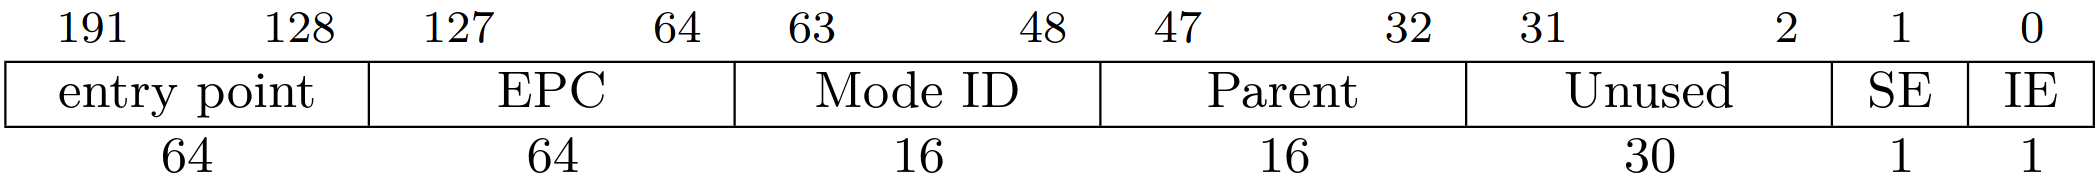
\includegraphics[width=\textwidth]{ue_entry}
    \caption{Mode descriptor}
    \label{fig:mode_desc}
\end{figure}


\subsection{Memory protection for Programmable modes}\label{chap:mem_perm}
A central focus of Von Elm's work involves devising a robust memory protection
mechanism tailored for software-based modes. He adopts a strategy that
split this task into two distinct components. The first task involves
tracking virtual page-to-physical page mappings, while the second task entails
determining access rights allocated to specific memory locations. Von Elm
justifies this partitioning by the potential impracticality of allocating
individual access bits for each mode in the Page Table Entries (PTEs) of a
conventional paging system, as it could lead to unwieldy and oversized PTEs.
However, this approach introduces the challenge of maintaining two separate
systems to accomplish what was previously handled within a single system.
Thus, both systems demand optimal performance for their respective tasks.\par
To address these challenges, Von Elm leverages the efficiency of the regular
paging system for the first task, which minimally impacts the translation
process. For the second task, he implements a segmentation-based approach.
This choice allows us to change permissions more fine-granular. This means it is
possible to use regions smaller than pages and regions that are not
page-aligned. By employing a segmentation model, it becomes possible to
encapsulate the access rights of an entire segment using a single segment
descriptor, rather than employing multiple page table entries (see Fig.\ref{fig:pag_seg}).\par 
\begin{figure}[h]
    \centering
    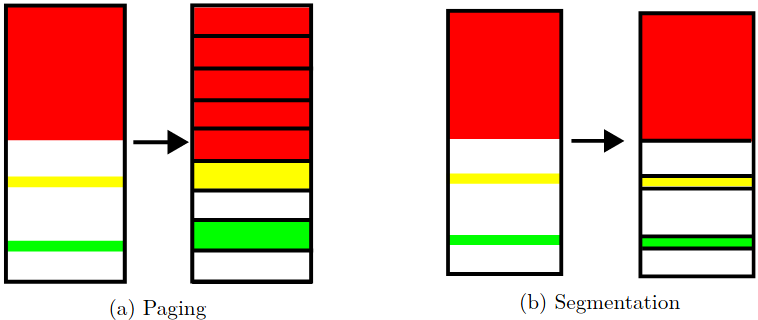
\includegraphics[width=\textwidth]{seg_pag}
    \caption{Paging and Segmentation compared}
    \label{fig:pag_seg}
\end{figure}
For the segmentation-based approach, Von Elm designs a so called
Permission-Lookaside-Buffer (PLB). During the translation phase, this PLB is
consulted to ascertain if a mode possesses permission to access a specific
memory region. Each PLB entry identifies the mode it corresponds to via a ModeID
field and defines the memory region through a start address and an offset,
specifying its size. Access rights are stored using the conventional read,
write, and execute bits, furnishing comprehensive control over memory access
(see Fig.\ref{fig:plb_desc}). This segmented approach offers an efficient means
of managing memory protection, striking a balance between performance and
granularity in access control for software-based modes.
\begin{figure}[h]
    \centering
    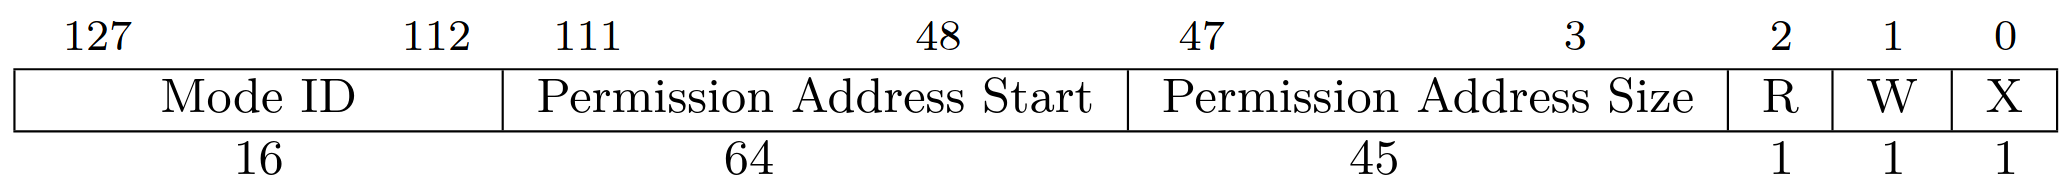
\includegraphics[width=\textwidth]{ue_plb}
    \caption{PLB descriptor}
    \label{fig:plb_desc}
\end{figure}